\cleardoublepage\chapter{Introduction}
\minitoc\label{sec:introduction}\vspace{.5cm}

\section{Background and Motivation}
A physical tunnel allows vehicles to move between 2 places independently from surrounding geography. 
Similarly, network tunneling is a mean to organize traffic between host A and B in a way that:

\begin{itemize}
    \item Abstracts the underlying path over the public network: Applications binding to the tunnel are not aware of the real paths that packets take.
    \item Encapsulates and encrypts: Middle man - even can intercept the traffic - can't always determine if a network frame belongs to the tunnel or a tunnel is being used, nor decrypt the content.
\end{itemize}

% A \ac{VPN} is a application build on top of a tunnel to connect 2 networks, effectively allow its host to access the other internal network remotely.
% Well known \ac{VPN} applications can be named: \ac{wgpage}, \ac{ovpnpage}, IPsec, PPTP, PPPoE, L2TP, ...
% Despite of the difference in level of operation (network or data link layer) and operation space (kernel or user space), they generally share the same concept of single link: the tunnel utilizes one single network link to transmit and receive the tunnel packets. 
A \ac{VPN} is an application that utilizes a tunnel to enable remote access to an internal network. 
Notable \ac{VPN} applications include \ac{wgpage}, \ac{ovpnpage}, IPsec, PPTP, PPPoE, L2TP, and more. 
Despite variations in their operational level (network or data link layer) and operation space (kernel or user space), these applications generally share the concept of using a single link for transmitting and receiving tunnel packets.
% The connection with support for \textit{multipath} concept, would deploy multiple network links so it can achieve higher reliability through redundancy or higher bandwidth through combining links, even though these characteristics are more relevant to environment such as infrastructure, data center or industrial application rather than end-user usage.
% There are protocols such as \ac{MPTCP}, \ac{SCTP} work this way, albeit in form of non-sharable connection.
% A non-share connection is initiated similarly to initiating a socket and can only be used by the caller program. 
% This severely limits the capability to control, schedule and share multipath resources between multiple applications in an effective manner, i.e prioritizing, buffering ... 
% These require centralized orchestration level of control over all communication channels by a control plane, which doesn't exist for these protocols.
A connection that supports the concept of \textit{multipath} utilizes multiple network links to enhance reliability through redundancy or increase bandwidth by combining links. 
% However, these characteristics are more applicable to environments such as infrastructure, data centers, or industrial applications rather than regular end-user usage. 
Protocols like \ac{MPTCP} and \ac{SCTP} operate in this manner, but they are implemented as non-sharable connections.
A non-share connection is initiated similarly to establishing a socket and can only be utilized by the program initiating it. This limitation severely restricts the ability to effectively control, schedule, and share multipath resources among multiple applications. 
Tasks such as prioritization and buffering become challenging without a centralized control plane that can orchestrate communication channels, which is currently absent in these protocols.
%
We propose another tunnel implementation: \ac{MTX}. 
% The tunnel will have multipath support by design, allow multiple applications to share the connection simultaneously, and be built based on Linux's \ac{xdppage} socket family.
% Using the latest native Linux's technology, the implementation is expected to performance-wise outperform any user space implementation while retain compatibility with existing systems and code base's simplicity. 
% Support for multiple connection links offers reliability, large raw-bandwidth and a rich set of configuration to applications binding to the tunnel, makes it suitable for high demand use-cases such as industry, data center, telecommunication hub. 
% In this document, an enhancement for the 5G's \ac{gptu} protocol \todo{cut this} with \ac{MTX} library will be investigated. \ac{gptu} is the protocol that helps UPF and gNodeB functions of a 5G system communicating, which demands both bandwidth and stability and therefore is a suitable match for a \ac{MTX} demonstration.
The tunnel is designed to support multipath capabilities and allow multiple applications to concurrently share the connection. 
It is constructed based on Linux's \ac{xdppage} socket family, leveraging the latest native Linux technology. 
This implementation is expected to outperform user space implementations in terms of performance while maintaining compatibility with existing systems and ensuring simplicity in the code base.
The support for multiple connection links offers reliability, high raw-bandwidth, and a comprehensive configuration set for applications bound to the tunnel. 
Consequently, it is well-suited for demanding use cases such as industry, data centers, and telecommunication hubs.
This document will investigate an enhancement for the 5G's \ac{gptu} protocol (Note: consider removing the "cut this" placeholder) using the \ac{MTX} library. 
The \ac{gptu} protocol facilitates communication between the UPF and gNodeB functions in a 5G system, demanding both bandwidth and stability. 
Therefore, it is an appropriate match for demonstrating the capabilities of the \ac{MTX} system. \todo{improve}
%

\begin{figure}[H]
	\centering
	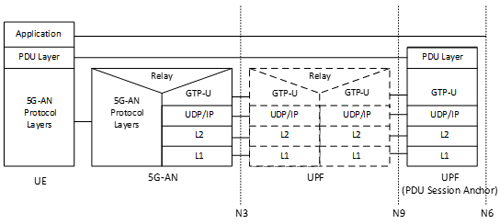
\includegraphics[width=0.8\textwidth]{resources/images/3gpp_5g_data_plane_protocol.png}
	\caption{3GPPP's 5G Data Plane protocol stack \cite{3gpp_5g_system_overview}}
    \label{fig:introduction:3gpp_5g_data_plane_protocol}
\end{figure}


\section{Problem Statement}\index{Requirements}\label{sec:introduction:problem_statement}
% In this section, the problems with single-link tunnel will be presented.
% Combine links
% The most commonly used technologies for communication in data center and \ac{HPC} environment are Ethernet and \ac{infinibandpage} (\Cref{fig:introduction:Interconnect_Technologies_500_supercomp}), which currently offer 100-200Gb/s bandwidth per line \cite{ethernet_roadmap}\cite{infiniband_roadmap}.
% These kind of bandwidth between computers (or inter-system) are nonetheless impressive, yet not comparable to the system's internal connection, i.e inter-chiplet bridge \textit{Infinity Fabric} used in AMD's Zeppelin SoC provides 256GB/s in-package bandwidth \cite{burd_zeppelin_2019}, and up to 800GB/s connection in GPUs peer-to-peer test \cite{amd_infinity_architecture}.
% This means even when invested in the current latest networking hardware, the connection between computer instances might be the bottleneck for certain applications that require distributed computation, for example large \ac{AI} or simulation model.
% In this case, a multipath tunnel can hide hide the multipath details of merging multiple links from the applications, effectively scales up the network capacity horizontally.
% The tunnel thus allow data center usage benefits from having larger combined bandwidth using current technology, but also is a necessary tool to overcome eventual physical and economical limitation in the future.
% For less demanding usages, aggregation is an affordable method to build fast connection from available hardware \todo{improve}.
Ethernet and InfiniBand are the most prevalent communication technologies in data centers and \ac{HPC} environments. 
Currently, these technologies provide bandwidths of 100-200Gb/s per line \cite{ethernet_roadmap}\cite{infiniband_roadmap} (\Cref{fig:introduction:Interconnect_Technologies_500_supercomp}). 
While this bandwidth is impressive for inter-system communication, it cannot match the internal connections within a system. 
For instance, AMD's "Infinity Fabric" bridge offers an in-package bandwidth of 256GB/s on Zeppelin SoC family \cite{burd_zeppelin_2019}, and up to 800GB/s in peer-to-peer tests between GPUs using more bands \cite{amd_infinity_architecture}.
This indicates that even with the latest networking hardware, the connection between computer instances can become a bottleneck for distributed data-intensive applications, for instance large \ac{AI} model or computer simulation. 
In such cases, a multipath tunnel can abstract the complexity of merging multiple links from the applications, effectively scaling up the network capacity horizontally. 
Consequently, the multipath tunnel enables data centers to benefit from larger combined bandwidth using current technology and serves as a necessary tool to overcome future physical and economic limitations.
For less demanding use cases, aggregation presents an affordable method to build fast connections using available hardware.
%
% Reliability
% Connection's reliability is closely related to the failure probabilities of the individual links and nodes (component reliability, can directly effect service availability) \cite{shooman_algorithms_1995} and the \ac{QoS} parameters \cite{gozdecki_quality_2003}.
% Common connection's \ac{QoS}  parameters can be named: latency, peak throughput, jitter.
% Depends on the use case, reliability of the connection can be a \ac{QoS} measurement factor (i.e commercial network provider) or a strict requirement (i.e critical application).
% Generally, 2 non-exclusive strategies are often used to increase a connection's reliability: through fortifying individual link, or redundancy.
% A connection's failure probability can be reduced by upgrading to a more resilient but expensive link or equipping with multiple failover lines. 
% Similarly, while better hardware can eliminate many \ac{QoS} inadequacy problems, having multiple links (or routes) each optimized for a type of appliance is certainly more suitable and affordable for the operator, especially if the data traffic is heterogeneous \cite{chen_overview_1998}.
% A multipath tunnel with flow-aware capability can be used in this case to manage the underlying links as an abstraction layer for the applications that utilize the connection. \todo{improve} \todo{more about QoS}
The reliability of a connection is closely tied to the failure probabilities of the individual links and nodes, which directly impacts service availability \cite{shooman_algorithms_1995}. 
Additionally, \ac{QoS} parameters such as latency, peak throughput, and jitter play a crucial role \cite{gozdecki_quality_2003}.
Depending on the use case, connection reliability can either serve as a \ac{QoS} measurement factor (e.g., for commercial network providers) or a strict requirement (e.g., for critical applications). 
Generally, there are two non-exclusive strategies commonly employed to enhance connection reliability: strengthening individual links or incorporating redundancy.
% Upgrading to more resilient, albeit costly, hardware links or implementing multiple failover lines can reduce the probability of connection failures. 
While superior hardware can reduce the probability of connection failures and address many \ac{QoS} inadequacies, having multiple links or routes optimized for specific applications is often a more practical and cost-effective approach for operators, particularly when dealing with heterogeneous data traffic \cite{chen_overview_1998}.
In such cases, a multipath tunnel with flow-aware capabilities can be utilized as an abstraction layer to manage the underlying links for applications relying on the connection. 
This allows for improved reliability and more effective utilization of resources. 
\todo{improve} \todo{more about QoS}

%  heterogeneous data traffic

%%
% Combine with a powerful CPU, networking application based on technologies such as \ac{dpdkpage} can saturate even a 100Gbit line using a single CPU core \cite{intel_dpdk_perf}. 
% However, this can be improved by combining bandwidth of many links. 
% A multipath tunnel will create a logical NIC for application, effectively abstracts the management, orchesteration tasks for the applications.
% \todo{sota: how these are being done in real life?}
% Such method can be useful for long term and short term usage: using existing technology and hardware to achieve higher bandwidth to reduce cost, and overcome physical limitation.

\begin{figure}[H]
	\centering
	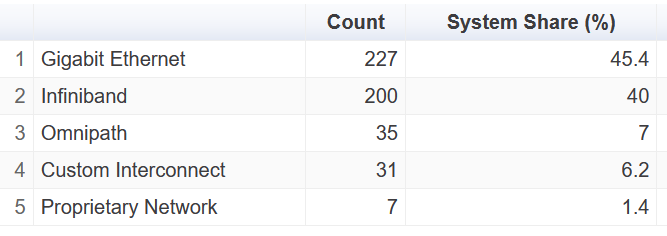
\includegraphics[width=0.8\textwidth]{resources/images/Interconnect_Technologies_500_supercomp.PNG}
	\caption{Interconnect technologies of top 500 super computers, 2023 edition as tracked by TOP500 project \cite{Interconnect_Technologies_500_supercomp}}
    \label{fig:introduction:Interconnect_Technologies_500_supercomp}
\end{figure}

\todo{other: latency, ...}

% Perf: userspace vs kernelspace process
% Omitting trivial tasks such as authentication and handshake, tunneling operation including the following steps: acquiration of ingress data stream (send to tunnel by application), process of ingress data (convert data into stream of tunnel packets, often through encapsulating with tunnel header, encrypting, compressing), and reverse on the receiving end (extrating original data from tunnel packets and delivering to application) \todo{cite+improve}.
% Apart from scaling the underlying system vertically (i.e by using more powerful hardware) or using a lower-level programing language, the most significant factor that could affect the performance of a single-link tunnel implementation is how ingress data is handled.


% \sidenote{State of the Art}
% \todomid{write about the State of the Art}

% \sidenote{Issue:\\Example 1}
% \todomid{write about the first issue}

% \sidenote{Issue:\\Example 2}
% \todomid{write about the second issue}

% \sidenote{Synopsis}
% \todomid{write about the synopsis of the issues and \Cref{fig:intro:c}}

% \begin{figure}[htbp]
%     \centering
%     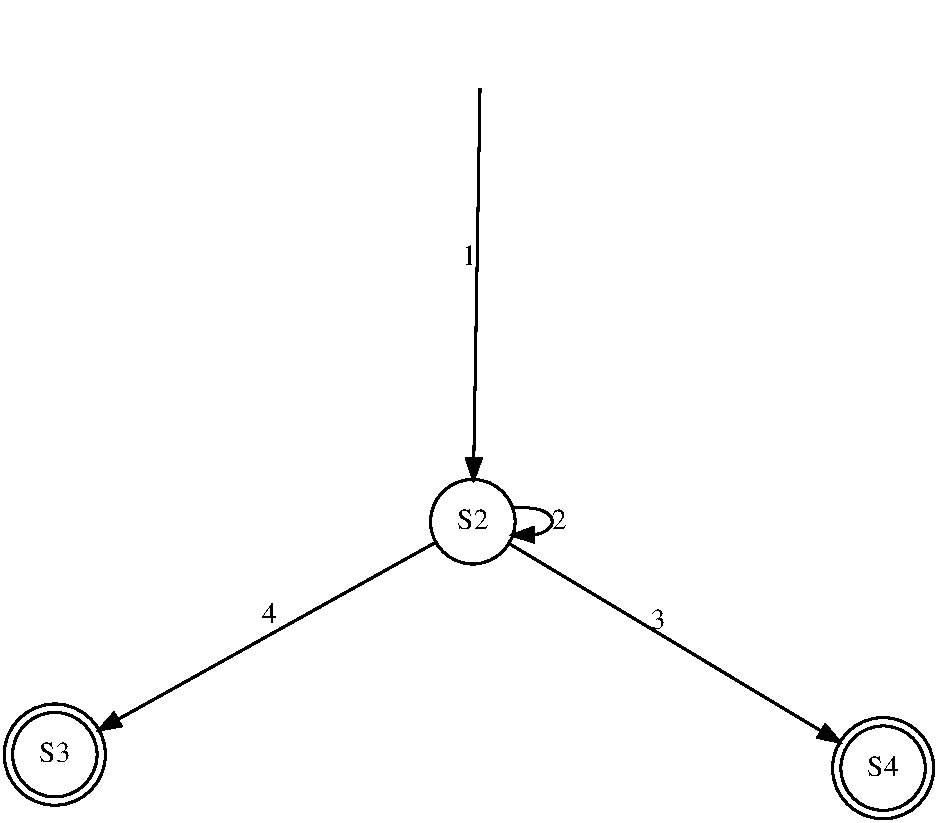
\includegraphics[width=.5\textwidth]{resources/images/job_lifecycle}
%     \caption{Relationship between issues}\label{fig:intro:c}
% \end{figure}

\section{Assumptions and Scope}

% \sidenote{Research Assumptions}
% \todomid{write about the research assumptions~\cite{li2002design}}
Besides the reliability's \ac{QoS} characteristic, we define the metrics to measure performance of a tunnel as follow:
\begin{itemize}
    \item Bandwidth: Quantity of data that can be transmitted through per second, usually measured in Megabit per Second (Mb/s) or Gigabit  per Second (Gb/s)
    \item Latency: Delay, measured in microsecond (us) or millisecond (ms). Latency introduced by the tunneling process at both ends compared to sending data over the same public path without the tunnel.
    \item System load: Tunneling process costs CPU time and RAM usage.
\end{itemize}

% The idea
The project is inspired by \ac{5G}'s \ac{NFV} and \ac{SDN} influenced specification.
Being recognized as the 2 technology enabler for realizing 5G networks, they allow concepts such as \textit{slicing} or \textit{decoupling} of hardware-software planes and control-data planes \cite{yousaf_nfv_sdn_key_techno_for_5g2017} \cite{open_baton} which make \ac{5G} a much more capable network standard than its predecessor while remains flexible and agile for operators \todo{better wording here}.
\ac{NFV} moves dedicated functions such as router, firewall that traditionally ran on dedicated hardware to virtualized environment and cloud-based infrastructure.
\ac{SDN} encourages using software based solution running on common hardware and software stack over conventional equipment and services which integrated on rigid hardware-based proprietary.
\ac{NFV} and \ac{SDN} thus helps reducing capital and operational expenditures, speeding up the release process and avoid vendor locking \cite{yousaf_nfv_sdn_key_techno_for_5g2017} \cite{sun_integrating_2015}.
These trends heavily influence the 5G infrastructure to employ recent software industry's practices, which include agile development, orchestration, moving to cloud, dynamic deployment, and \ac{HA} through horizontal partition.
\ac{5G}'s distributed network services and diverse \ac{QoS} require reliable and high throughput connection, which as discussed in \Cref{sec:introduction:problem_statement} can be horizontally implemented in an performant and cost-effective way using multiple links instead of vertical scaling paradigm.

% building block:
Moving functions to cloud and virtual environment faces performance challenges, one of which is the overhead introduced by the abstraction, virtualization layers as well as the extra input/output and communication between functions that can be found locally before \cite{yousaf_nfv_sdn_key_techno_for_5g2017}.
Although the running newly designed cloud-native software on orchestrated thin containers help addressing the performance problem, we believe some aspects of the connection can be improved further, namely compatibility and ease of development and deployment.
In many 5G's implementation, technologies such as \ac{dpdkpage} and \ac{sriov} are being used to deliver line-speed packet processing capability to hypervisor environment with minimal impact on system performance \cite{intel_dpdk_perf} \cite{openstack_sriov} \cite{zte_5g_core_upf_impl} \cite{nec_hite_paper_upf_perf}.
We believe that these technologies proved their worthy, yet the systems suffer from limitation such as special requirement and configuration \todo{cite, that dpdk and sriov can't run on all commercial system}.
This would not only increase cost, but also make the product less attractive for research and test bed purposes, especially in the open source and academy community where budget and custom support is limited.
To address this, using a native and more simple Linux's technology - \ac{xdppage}, a new socket family based on eBPF technology with comparable performance to \ac{dpdkpage} - to build a tunnel that is designed to support multipath and multi-flow could be a promising supplement for existing implementation. \todo{more}


% \sidenote{Research Scope}
% \todomid{write about the research scope --- \Cref{fig:intro:a,fig:intro:b,fig:intro:c}}
With an implementation and a thesis documentation for the multipath tunnel as the desire outcome of the project , we define the scope of the project as followed:
\begin{itemize}
    \item Scope of research: this research is limited to investigating a tunnel implementation based on \ac{xdppage} technology that employs multipath and flow-aware concepts. A functional tunnel is expected to be built in 3 months. From there, more complex features will be added along with a test application to run on top the tunnel for testing and demonstrating purposes. In the course of building process, this initiated documentation will be updated until the project reaches its time limitation (6 months in total). Although the tunnel library will be a general purpose framework that can be deployed for any application, it is intended to be tested with 5G's software stack in mind.
    \item Foreseeable tasks: researching the project idea, building multipath protocol, implementing the tunnel, testing and demonstrating tasks are planed. 
    \item Implementation: the tunnel will be implemented in C/C++, uses \ac{xdppage} sockets as the packet transport layer. The tunnel shall be able to exchange data over multiple \ac{NIC}s and treat each packet differently based on defined configuration (stream based/flow based). More will be discussed in the next section.
    \item Demonstration: used to test and present the features of the tunnel. At this stage, a simplified version of \ac{gptu} protocol has been chosen to run on top of the tunnel. \ac{gptu} is the communication protocol responsible for establishing data exchanging channels in 5G's \ac{UPF} and gNodeB. These channels (or tunnels) handle streams of data, each has \ac{QoS} identifier with different characteristics and priority. This makes the protocol a good match for tunnel demonstration purpose.
\end{itemize}


\section{Objectives and Contributions}
The research is limited to investigating the multipath concept with a new technology. 
Generally, the tunnel implementation can be useful for the following scenarios:
\begin{itemize}
    \item High bandwidth connection for High performance computing, servers, data center.
    \item High reliability for critical application by using backup links for tunnel or replicate packets.
    \item 5G back-haul and middle-haul: power the forwarding/relaying mechanism (\ac{UPF}, gNodeB's UD-CU). Enhance existing GTP-U protocol with multipath, flow-aware capability.
\end{itemize}

Although we hope the project's outcome can contribute to the general understanding of software based solution for high performance networking field, we seek opportunity to integrate the tunnel into the next generation telecommunication system. We found 2 potential improvements according to our research: \todo{improve the following text}
\begin{itemize}
    \item N6 connection between UPF (also N9 i.e between UPF-E and UPF-C) and Data network: enhanced by prioritized, flow-aware, high bandwidth multipath tunnel. To meet differentiated SLA requirements for latency, bandwidth and reliability, UPF needs to be deployed at different positions including central DC, regional DC, edge DC and campus DC. MTX can help saturating physical links coup with support large number of UEs.
    \item 5G user plane (back-haul N3 between gNodeB-UPF, mid-haul between gNodeB-CU and -DU) relied on message-based protocol \ac{gptu} (the character "U" means "user data tunneling") to relay traffic in tunnels - or flows within a PDP session.
\end{itemize}

We also identified reports regarding performance issues in the \ac{UPF} of \ac{o5gs} - a well-known 5G core implementation that the AV team at the TU Berlin is currently using in their 5G test bed. Contributors have proposed employing \ac{dpdkpage} and exploring lower-level approaches to minimize overhead \cite{open5gs_github_dpdk}\cite{open5gs_github_udp_perf_cap}, as the current implementation limits the TUN interface bandwidth to 1Gbit. We believe that through thorough analysis, this presents an opportunity for us to make a valuable contribution to the \ac{o5gs} project with our MTX tunnel.

\begin{figure}[H]
	\centering
	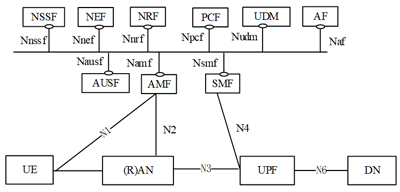
\includegraphics[width=0.8\textwidth]{resources/images/3gpp_5g_system_overview.png}
	\caption{3GPP's 5G System Overview \cite{3gpp_5g_system_overview}}
    \label{fig:introduction:3gpp_5g_system_overview}
\end{figure}


% \begin{figure}[htbp]
%     \centering
%     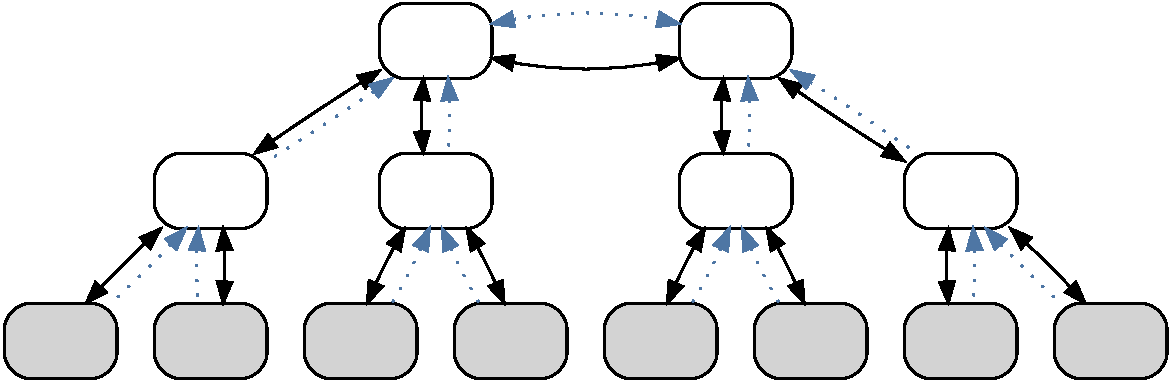
\includegraphics[width=.55\textwidth]{resources/images/example3}
%     \caption{Structure of research}\label{fig:intro:struct}
% \end{figure}

% \sidenote{Research Objectives \& Contributions}
% \todomid{write about the research objectives and \ac{DBpedia} and \Cref{fig:intro:struct}}

% \section{Methodology and Outline}

% \todomid{write about the research outline and \Cref{fig:intro:methodology}. Summarize \Cref{sec:introduction,sec:sota,sec:reqs,sec:contrib1,sec:contrib2,sec:contrib3,sec:eval,sec:summary}.}

% \begin{sidewaysfigure}
%     \centering
%     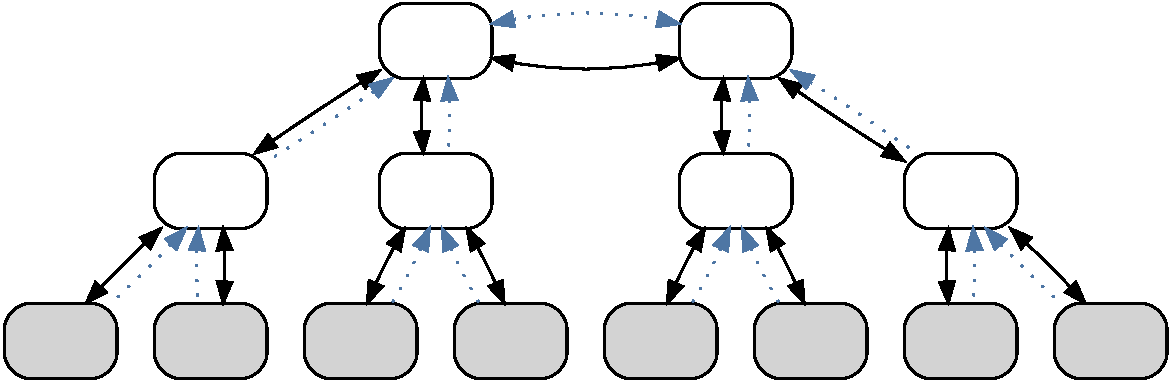
\includegraphics[width=.7\textwidth]{resources/images/example3}
%     \caption{Workflow of the research and structure of the thesis}\label{fig:intro:methodology}
% \end{sidewaysfigure}
